\begin{frame}
	\frametitle{Herramientas Software}
	\block{{\it Android Studio}: \texttt{http://developer.android.com/sdk}}
		\begin{itemize}
			\item Entorno de desarrollo integrado.
			\item Uso intuitivo.
			\item Ligero.
		\end{itemize}
	\endblock{}
	\vfill 
	\begin{center}
		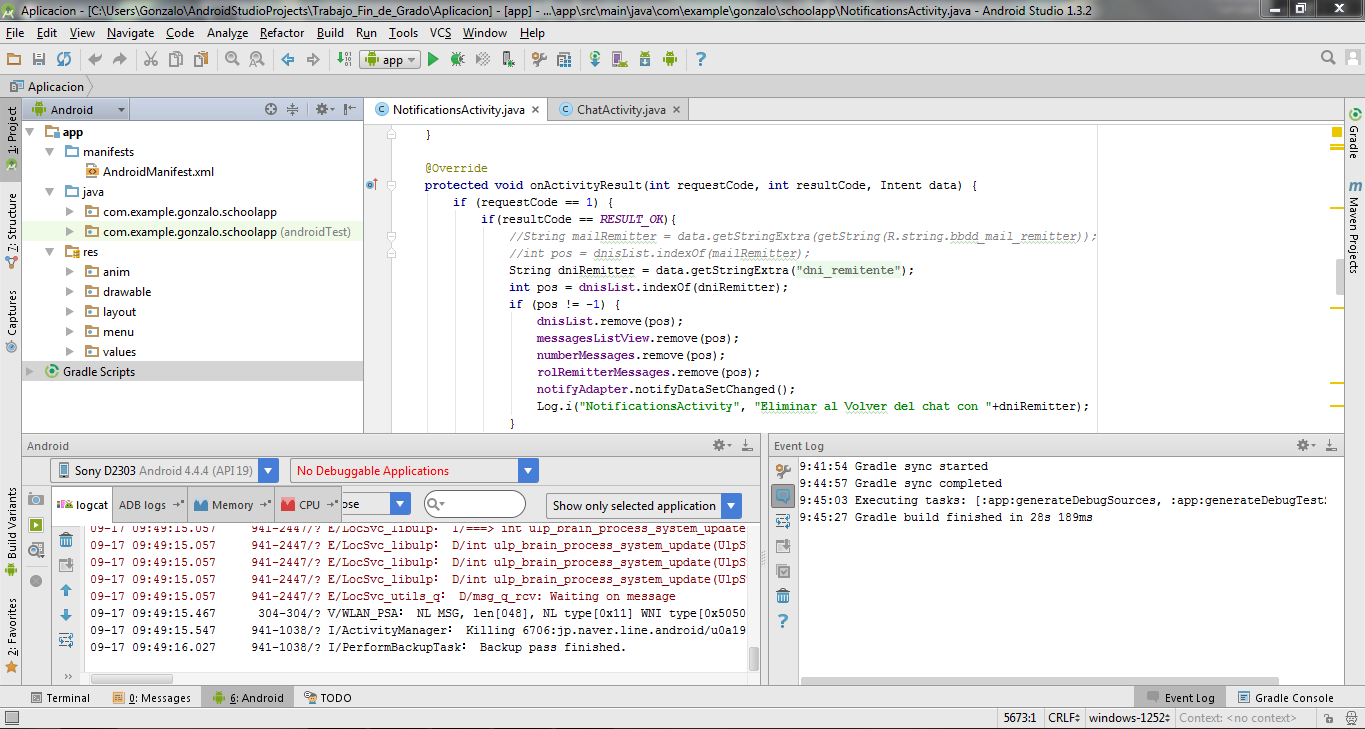
\includegraphics[width=0.8\linewidth]{Images/AndroidStudio}
	\end{center}
\end{frame}

%------------------------------------------------------------------
\begin{frame}
	\frametitle{Herramientas Software}
	\block{\it Tutoriales de Android Studio}
		\begin{itemize}
			\item {\it Suporting different devices}.
			\item {\it Building a dynamic UI with fragments}.
			\item {\it ActionBar Tab Swipe}.
			\item {\it TabHost Swipe}.
			\item {\it Adding animations}.
			\item {\it Expandable ListView}.
		\end{itemize}
	\endblock{}
\end{frame}

%------------------------------------------------------------------

\begin{frame}
	\frametitle{Herramienta Software}
	\begin{columns}
		\begin{column}{0.6\textwidth}
			\block{\it Firebase}
			\begin{itemize}
				\item Proveedor de contenidos.
				\item Ofrece servicios en la nube.
				\item Seguro y sencillo (Funcionalidades).
				\item Datos tipo JSON.
				\item Consturucción de datos en tiempo real.
				\item Interfaz de programación de aplicaciones de seguridad basada en la expresión altamente flexible.
			\end{itemize}
			\endblock{}
		\end{column}
		\begin{column}{0.4\textwidth}
			\vfill 
			\begin{center}
				
\includegraphics[width=0.8\linewidth]{Images/logos/firebase_logo}
			\end{center}
		\end{column}
	\end{columns}
	\block{\it Tutorial}
		\begin{itemize}
			\item {\it Firebase Storage}: \\ {\texttt{https://www.firebase.com/docs/android/guide/}}
		\end{itemize}
	\endblock{}
\end{frame}

%------------------------------------------------------------------

\begin{frame}
	\frametitle{Interacción con la base de datos en {\it Firebase}}
	\block{Base de datos en la nube}
	\begin{enumerate}
		\item En {\ttfamily app/build.gradle} añadir:
		\begin{itemize}
			\item {\ttfamily compile 'com.firebase:firebase-client-android 2.2.1'}
		\end{itemize}
		\item Importar los servicios a usar en los archivos de clase ({\ttfamily java}).
		\item  En {\ttfamily onCreate()} incorporar:
		\begin{itemize}
			\item {\ttfamily Firebase.setAndroidContext(this)}
		\end{itemize}
		\item Colocar una referencia a la base de datos o a una de sus tablas.
		\item Crear la consulta.
		\item situar un {\it oyente} ({\ttfamily listener}).
	\end{enumerate}
	\endblock{}
\end{frame}

%------------------------------------------------------------------

\begin{frame}
	\frametitle{Ejemplo interacción con la base de datos (Obtener datos)}
	\lstinputlisting{Code/StudentActivity.java}
\end{frame}

%--------------------------------------------------------------------

\begin{frame}
	\frametitle{Ejemplo interacción con la base de datos (Almacenar datos)}
	\lstinputlisting{Code/AddChildActivity.java}
\end{frame}

%--------------------------------------------------------------------

\begin{frame}
	\frametitle{Herramientas Software}
	\begin{columns}
		\begin{column}{0.6\textwidth}
			\block{\it Parse}
			\begin{itemize}
				\item Proveedor de servicios en la nube.
				\item Alternativa a {\it Firebase}.
				\item Utiliza datos SQL.
				\item Múltiples SDK.
				\item Notificaciones tipo {\it Push}.
			\end{itemize}
			\endblock{}
		\end{column}
		\begin{column}{0.4\textwidth}
			\vfill 
			\begin{center}
				
\includegraphics[width=0.9\linewidth]{Images/logos/parse_logo}
			\end{center}
		\end{column}
	\end{columns}
	\block{\it Tutorial}
		\begin{itemize}
			\item {\it Parse Storage}:\\ {\texttt{http://www.sitepoint.com/creating-cloud-backend-android\\-app-using-parse/}}
		\end{itemize}
	\endblock{}
\end{frame}